\documentclass[a4paper, 11pt, twoside]{scrreprt}
\usepackage[inner=3.5cm,outer=2.5cm,top=2.5cm,bottom=2.5cm,includeheadfoot]{geometry}

%\usepackage[utf8]{inputenc} %fuer Linux
\usepackage[latin1]{inputenc}

\usepackage{textcomp}
\usepackage[T1]{fontenc}
\usepackage[USenglish]{babel}
\usepackage{amsmath}
\usepackage{graphicx}
\usepackage[onehalfspacing]{setspace}
\usepackage{nameref}
\usepackage[bf]{caption}
\usepackage[hyphens]{url}
\usepackage{multirow}

%\usepackage{C://Users/Guinivere/Documents/GitHub/PhD/ReleaseNote/jenny}
\usepackage{jenny}

% \def\UrlBreaks{\do\a\do\b\do\c\do\d\do\e\do\f\do\g \do\h\do\i\do\j\do\k\do\l%
% \do\m\do\n\do\o\do\p\do\q\do\r\do\s\do\t\do\u\do\v \do\w\do\x\do\y\do\z\do\0%
% \do\1\do\2\do\3\do\4\do\5\do\6\do\7\do\8\do\9\do\-}%+
\usepackage[breaklinks=true]{hyperref}
\usepackage[title, titletoc]{appendix}




\usepackage{fancyhdr}



\fancypagestyle{empty}{
        \fancyhead{} % clear all header fields
        \fancyfoot{} % clear all header fields
        \renewcommand{\headrulewidth}{0pt}
        \renewcommand{\footrulewidth}{0pt}
}

\fancypagestyle{plain}{
        \fancyhead{} % clear all header fields
        \fancyfoot{} % clear all footer fields
        \fancyfoot[LE,RO]{\thepage}
        \fancyfoot[LO]{{\small Jennifer P\"{u}tz}}
        \fancyfoot[RE]{{\small Forschungszentrum J\"{u}lich}}
        \renewcommand{\footrulewidth}{0.4pt}
}
\pagestyle{fancy}
\fancyhead{} % clear all header fields
\fancyhead[RO]{\bfseries \slshape \nouppercase \rightmark} %\bfseries
\fancyhead[LE]{\bfseries \slshape \nouppercase \leftmark} %\bfseries
\fancyfoot{} % clear all footer fields
\fancyfoot[LE,RO]{\thepage}
\fancyfoot[LO]{{\scriptsize Jennifer P\"{u}tz}}
\fancyfoot[RE]{{\scriptsize Forschungszentrum J\"{u}lich}}



\renewcommand{\theequation}{\thesection .\arabic{equation}}
\renewcommand{\thefootnote}{[\arabic{footnote}]}
\renewcommand{\footnotesize}{\scriptsize}
%\renewcommand{\captionfont}{\footnotesize}
\renewcommand{\appendixname}{Anhang}



\setlength{\footnotesep}{8pt}
\setlength{\headheight}{1.1\baselineskip}


\begin{document}
	\pagestyle{fancy}
	\begin{titlepage}
		\thispagestyle{empty}
		\begin{center}
			\textbf{\Huge{Study of Excited \cascade Baryons in \pbarpSystem-Collisions with \panda}}\vspace{1cm}\\
			\Large{Authors:}\vspace{0.3cm}\\
			\LARGE{\underline{Jennifer 
			      P\"{u}tz}, Albrecht Gillitzer, James Ritman\vspace{2cm}}
		\end{center}\vspace{1cm}

	\end{titlepage}
	\thispagestyle{empty}
	%\cleardoublepage
	\chapter*{Abstract}
		Understanding the excitation pattern of baryons is indispensable for a deep insight into the mechanism of non-perturbative QCD. 
Up to now only the nucleon excitation spectrum has been subject to systematic experimental studies while very little is known 
on excited states of double or triple strange baryons.

\noindent In studies of antiproton-proton collisions the \panda experiment is well-suited for a comprehensive baryon spectroscopy program
in the multi-strange and charm sector. 
A large fraction of the inelastic \pbarpSystem cross section is associated to final states with a baryon-antibaryon pair together with 
additional mesons, giving access to excited states both in the baryon and the antibaryon sector.

\noindent In the present study we focus on excited \cascade states. For final states containing a \cascade\anticascade pair cross sections 
up to the order of $\mu$b are expected, corresponding to production rates of $\sim 10^6/$d at a Luminosity $L=10^{31} \unit{cm}^{-2} \unit{s}^{-1}$
 ($5\%$ of the full value).
A strategy to study the excitation spectrum of \cascade baryons in antiproton-proton collisions will be discussed. The reconstruction of 
reactions of the type \pbarpSystem $\rightarrow \Xi^{*}$ \anticascade (and their charge conjugated) with the \panda detector will be presented 
based on a specific exemplary reaction and decay channel.
	
	%
	\pagenumbering{Roman}
	\tableofcontents
	\newpage
	\pagenumbering{arabic}
	\setcounter{page}{1}

	\chapter{Motivation}
	
	\chapter{Event generation}
		To study excited \cascade baryons the simulation of signal events is needed.
For this study\\ 1.5 million signal events have been generated.
The decay channel for the simulation is shown in figure \ref{fig:eventgeneration_decaychannel}. 

\begin{figure}[htbp]
	\centering
			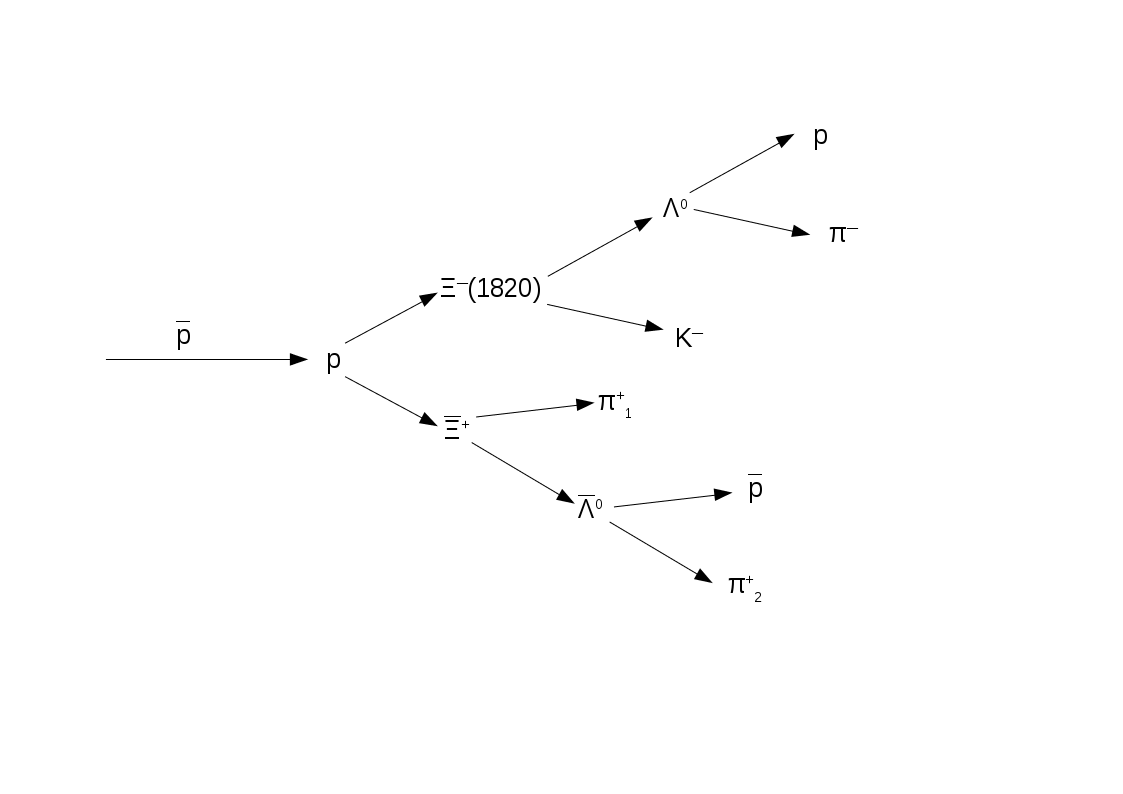
\includegraphics[width=1.00\textwidth]{./plots/DecayChannelXi1820.png}
	\caption{Simulated decay channel}
	\label{fig:eventgeneration_decaychannel}
\end{figure}

For the charge conjugated channel another 1.5 million events were generated.
Table \ref{tab:eventgeneration_parameter} shows the parameters which are used for the event generation.

\begin{table}[tbp]
	\caption{Parameter for event generation}
	\label{tab:eventgeneration_parameter}
	\centering
	\begin{tabular}{ll}
		\hline
		Parameter & Value \\
		\hline
		\hline
		Beam momentum & 4.6 \massunit \\
		Production & PHSP \\
		Tracking & Ideal \\
		Particle ID & Ideal \\\hline
		 
	\end{tabular}
\end{table}

The PHPS model is used for the production, because other models are not tested yet. 
But this is not effecting the strategy for this study.

The chosen beam momentum of $p_{\bar{\mt{p}}} = 4.6\unit{GeV/c}$ is 100 MeV above the production threshold of \excitedcascade and \anticascade.
The production cross section is expected to be of the same order ($\sim \mu\mt{b}$) as for \cascade \cite{PANDAphysics2009}.\\
\vspace{11pt} 

The used software versions for PandaRoot and the external software package is listed in table \ref{tab:eventgeneration_software} 

\begin{table}[tb]
	\centering
	\caption{Used software versions}
	\label{tab:eventgeneration_software}
	\begin{tabular}{ll}
		\hline
		Software & Version \\
		\hline
		\hline
		FairSoft & mar15\\
		FairRoot & v-15.03a \\
		PandaRoot & trunk revision 28555 \\
		Geant & 3\\
		Genfit & 1\\\hline
			 
	\end{tabular}
\end{table}


Since now \excitedcascade was not defined in the evt.pdl file. 
How the particle is added to the file is shown in the code snippet \ref{lst:eventgeneration_evtpdl}.
The properties of \excitedcascade are listed in table \ref{tab:eventgeneration_Xivalues}.

\begin{lstlisting}[caption={snippet from evt.pdl}\label{lst:eventgeneration_evtpdl}, captionpos=t,breaklines=true]
add  p Particle Xi(1820)- 23314 1.8230000e+00 2.4000000e-02 2.0000000e-01 -3 3 0.0000000e+00 23314
add  p Particle anti-Xi(1820)+ -23314 1.8230000e+00 2.4000000e-02 2.0000000e-01 3 3 0.0000000e+00 -23314
\end{lstlisting}

\begin{table}[htbp]
	\centering
	\caption{Properties of \excitedcascade and \excitedanticascade. The values are taken from \cite{PDG}}
	\label{tab:eventgeneration_Xivalues}
	\begin{tabular}{lllllll}
		\hline
		Particle & J & I & P & Charge & Mass  & Width \\
		\hline
		\hline
		&&&&&&\\
		\excitedcascade & $\frac{3}{2}$ & $\frac{1}{2}$ & ($-1$) & ($-1$) & ($1.823 \pm 5$)\massunit & ($0.024 \pm 6) $ GeV \\
		\excitedanticascade & $\frac{3}{2}$ & $\frac{1}{2}$ & ($-1$) & 1 & ($1.823 \pm 5$)\massunit & ($0.024 \pm 6) $ GeV\\
		\hline
		  
	\end{tabular}
\end{table}

The generated transverse momentum against the longitudinal momentum for \lam, \alam, \anticascade and \excitedcascade is 
presented in figure \ref{fig:MC_lambda0_pt_vs_pz}% -- \ref{fig:MC_xi_pt_vs_pz}.\\


\begin{figure}
	\subfigure[\lam]{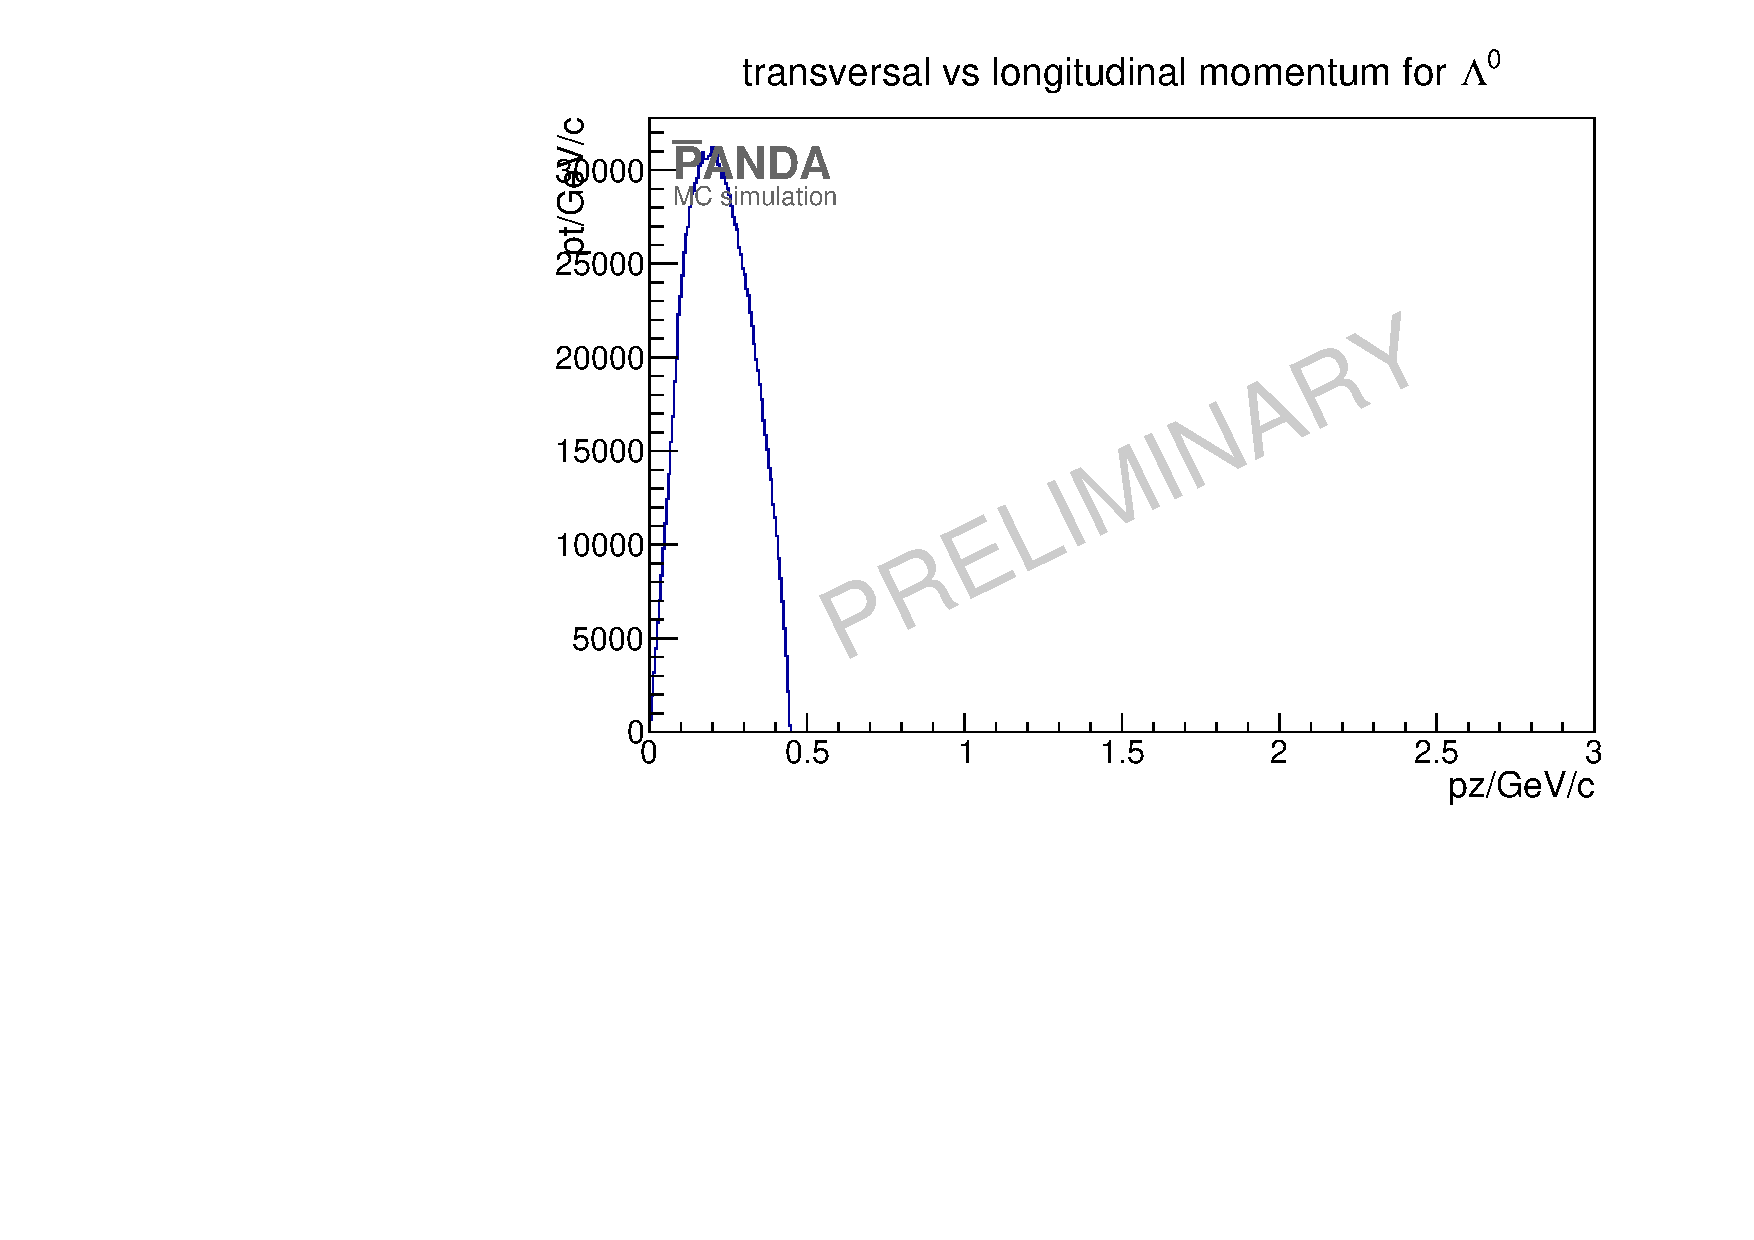
\includegraphics[width=0.49\textwidth]{./plots/lambda0/Lambda0_MC_pt_vs_pz.pdf}}
	\subfigure[\alam]{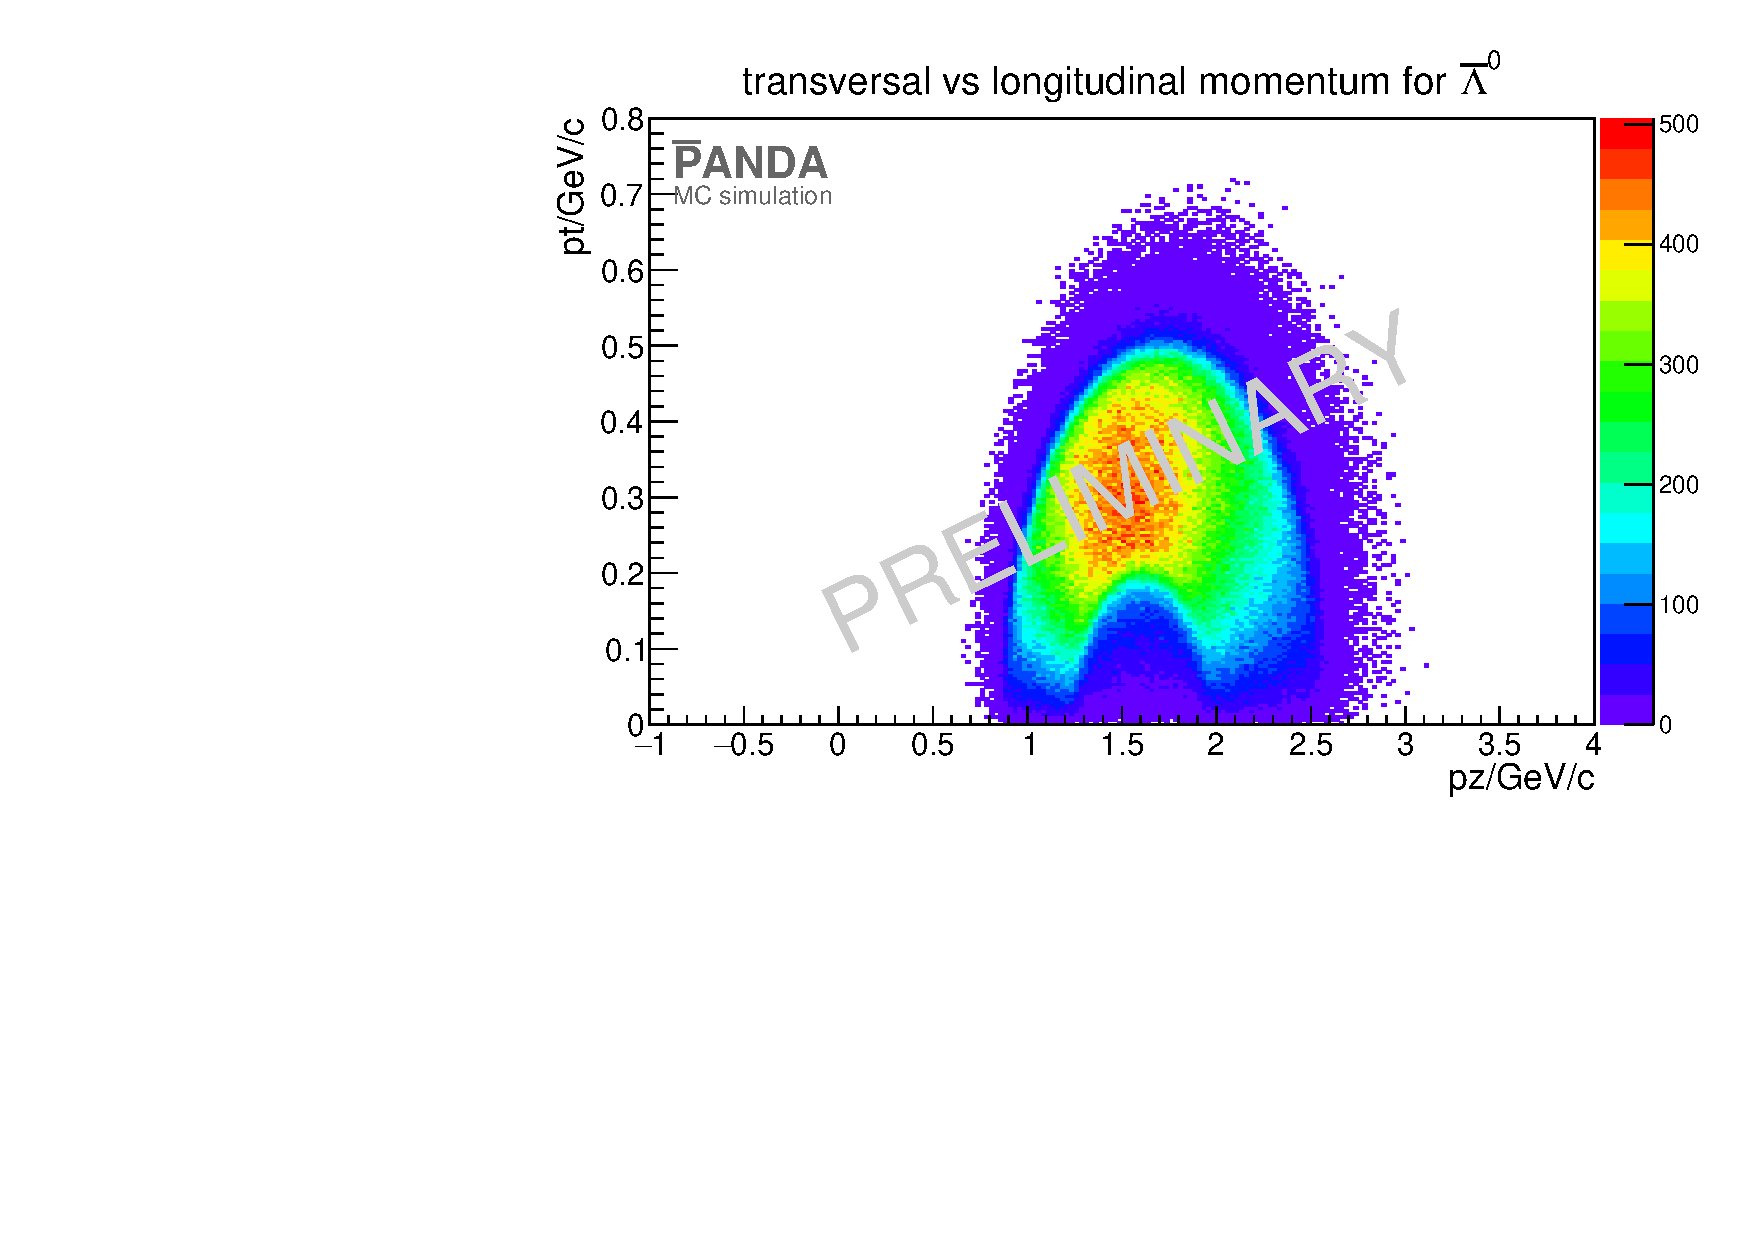
\includegraphics[width=0.49\textwidth]{./plots/antilambda0/AntiLambda0_MC_pt_vs_pz.pdf}}
	\caption{\propose Figure a) shows the transverse momentum on the y axis against the longitudinal momentum on the x axis for \lam. Figure b) 
			shows the same distribution for \alam.}
	\label{fig:MC_lambda0_pt_vs_pz}
\end{figure}


\begin{figure}
	\subfigure[\anticascade]{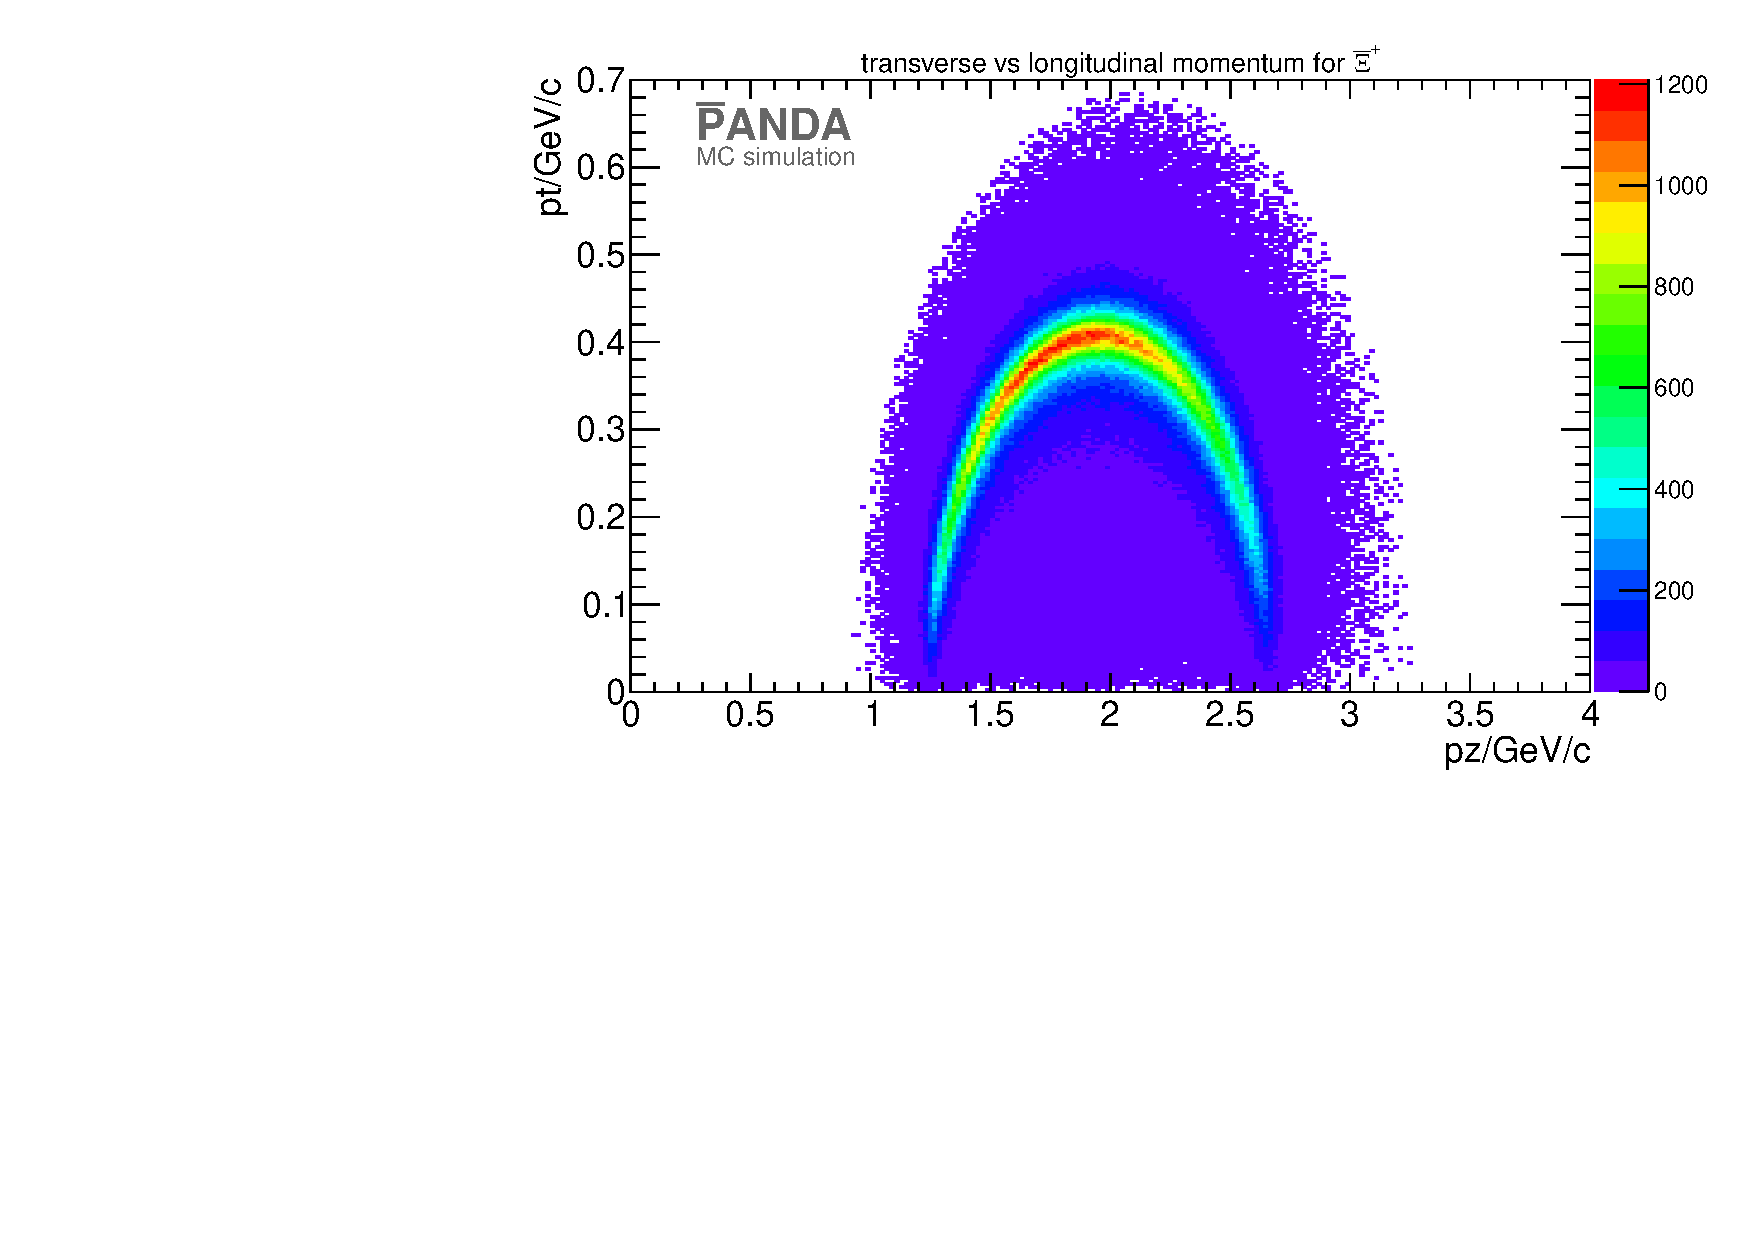
\includegraphics[width=0.49\textwidth]{./plots/Xi/XiPlus_MC_pt_vs_pz.pdf}}
	\subfigure[\excitedcascade]{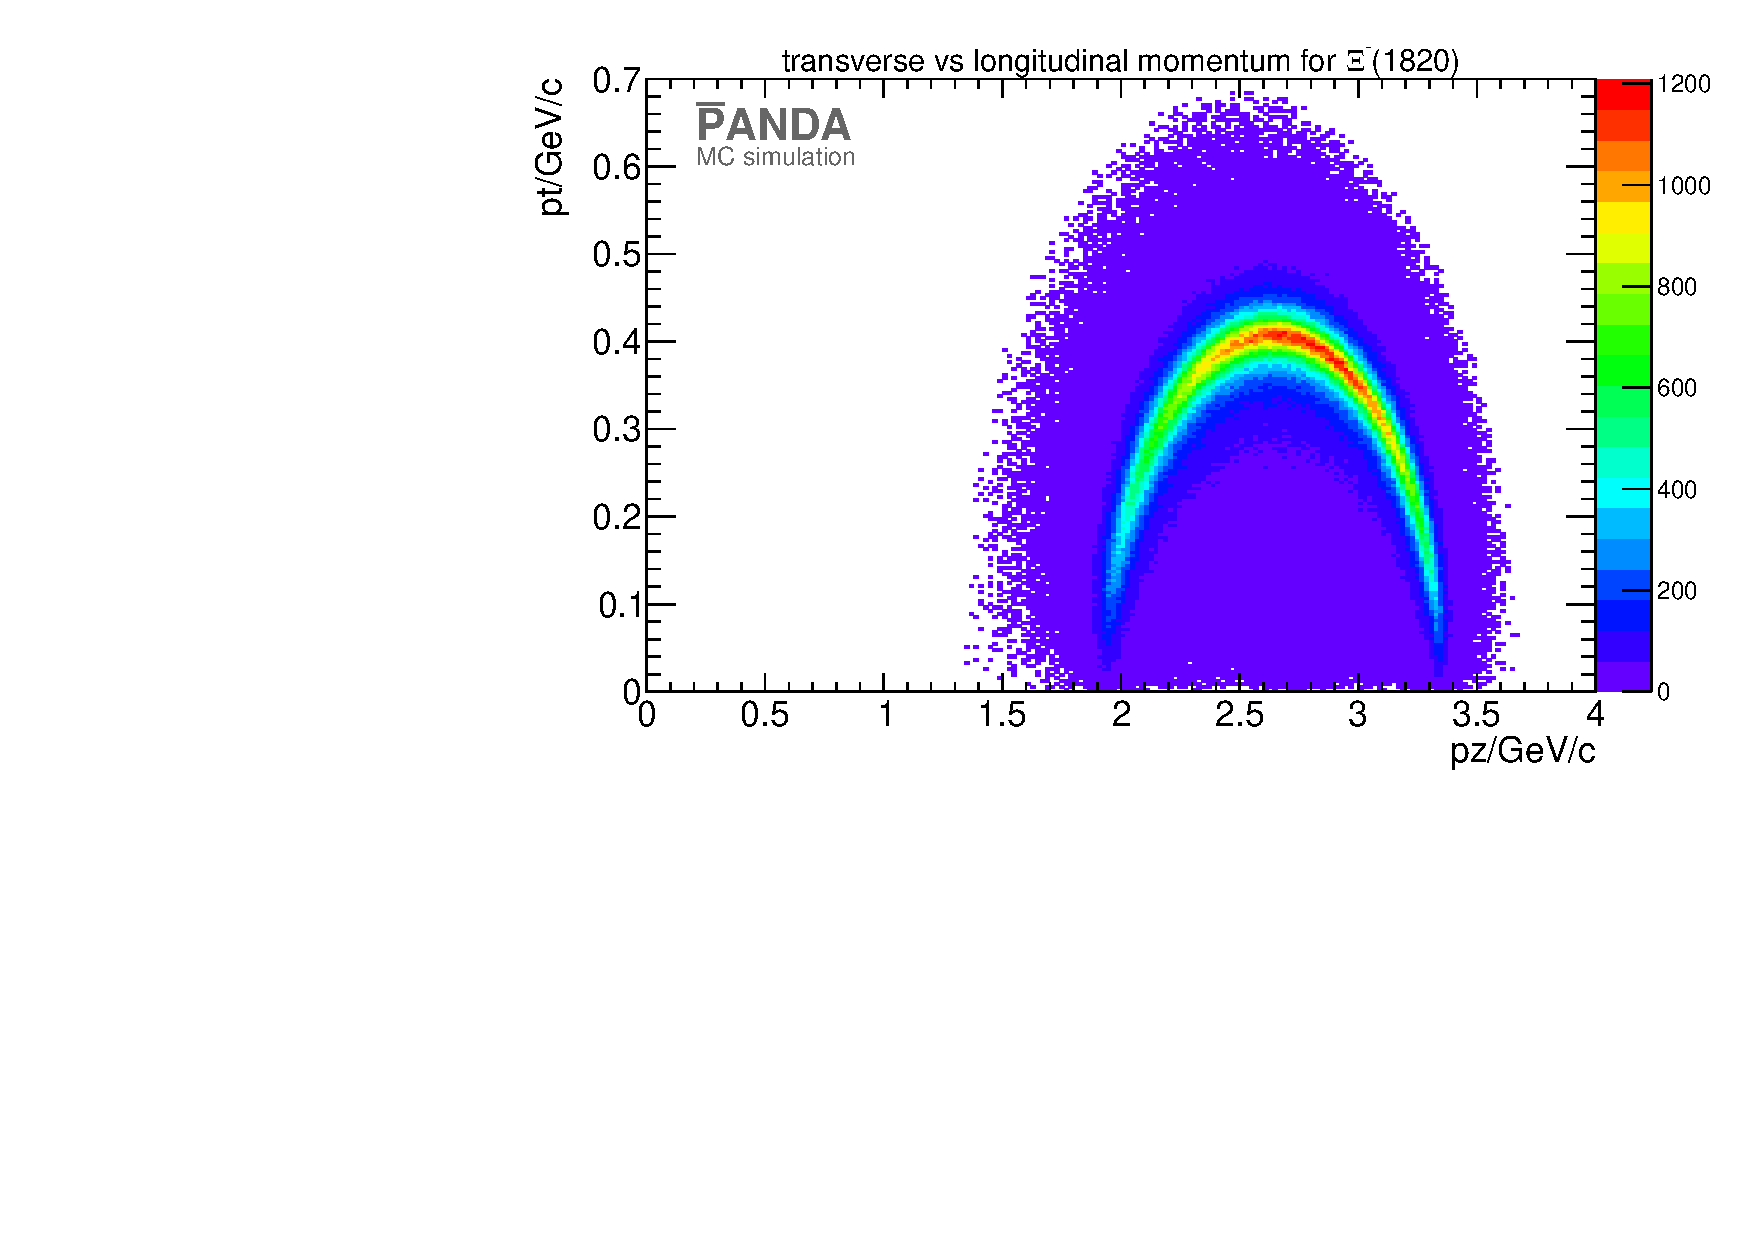
\includegraphics[width=0.49\textwidth]{./plots/Xi1820/XiMinus1820_MC_pt_vs_pz.pdf}}
	\caption{\propose Figure a) shows transverse against the longitudinal momentum distribution for \anticascade. Figure b) 
			transverse versus longitudinal momentum distribution for \excitedcascade.}
	\label{fig:MC_xi_pt_vs_pz}
\end{figure}

Figure \ref{fig:eventgeneration_Dalitz} shows the Dalitz plot for the \lam, \kminus and \anticascade final states for 
the channel \pbarpSystem $\rightarrow$ \excitedcascade \anticascade. 

\begin{figure}
	\centering
	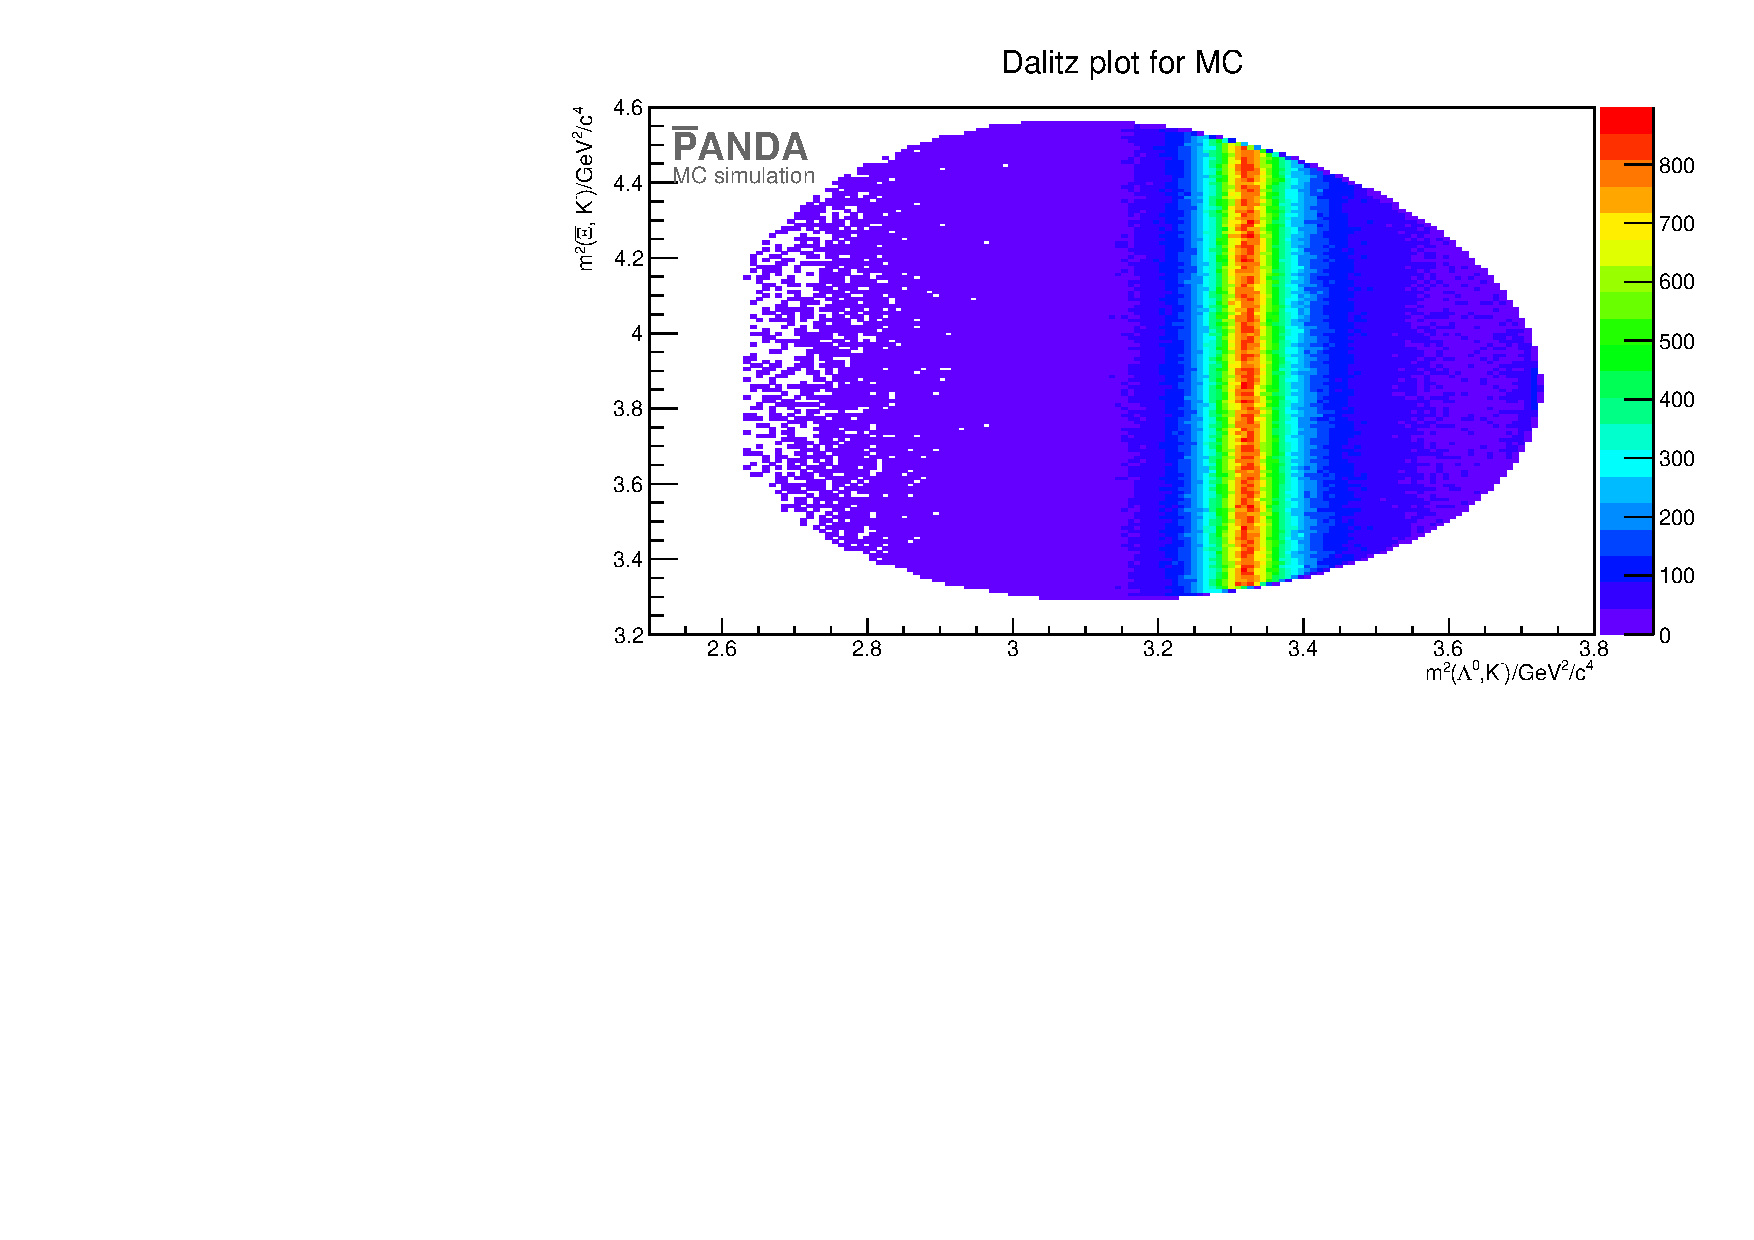
\includegraphics[width=0.6\textwidth]{./plots/Dalitzplot_MC.pdf}
	\caption{\propose Dalitz plot for simulation. On x axis is the mass square of \lam  and \kminus and on the y axis there is the mass square of \anticascade and \kminus}
	\label{fig:eventgeneration_Dalitz}
\end{figure}


	
	\chapter{Analysis}
	
	\chapter{Background}
	
	
	%\begin{appendices}
	%\fancyhead[RO]{\bfseries \slshape \nouppercase \rightmark} %\bfseries
	%\fancyhead[LE]{\bfseries \slshape \nouppercase Anhang A} %\bfseries
	%\renewcommand{\thesection}{\Alph{section}}
	%\setcounter{section}{0}
	%\chapter*{Anhang}
	%\addcontentsline{toc}{chapter}{ }
	%\end{appendices}
	%
	%\clearpage
	%\phantomsection
	%\addcontentsline{toc}{chapter}{Abbildungsverzeichnis}	
	%\fancyhead[RO]{\bfseries \slshape \nouppercase \rightmark} %\bfseries
	%\fancyhead[LE]{\bfseries \slshape \nouppercase \leftmark} %\bfseries
	%\listoffigures	
	%\listoftables
	%\addcontentsline{toc}{chapter}{Tabellenverzeichnis}
 	%\fancyhead[RO]{} %\bfseries
 	%\fancyhead[LE]{\bfseries \slshape \nouppercase Literaturverzeichnis} %\bfseries
	%\bibliography{literaturverzeichnis}
	%\bibliographystyle{alpha}
	%\addcontentsline{toc}{chapter}{Literaturverzeichnis}


\end{document}
